\documentclass[a4paper]{article}
\usepackage{graphicx}
\usepackage{multicol}
\usepackage{pdfpages}
\usepackage{pax}
\usepackage[none]{hyphenat}
\usepackage[cm]{fullpage}
\usepackage{attachfile}
\usepackage[utf8]{inputenc}
\usepackage{fancyhdr}

\DeclareUnicodeCharacter{00A0}{~}

\pagestyle{fancy}
\fancyfoot{}
\fancyfoot[C]{CITES Species Index – \thepage}
\renewcommand{\headrulewidth}{0pt}

\iftrue
  \usepackage{hyperref}
  \hypersetup{
    colorlinks=true,
  }
\fi

\begin{document}

\renewcommand{\rmdefault}{phv}
\newcommand{\superscript}[1]{\ensuremath{^{\textrm{#1}}}}
\newcommand{\cpart}[1]{\addcontentsline{toc}{part}{#1}\part*{\centering #1}}
\newcommand{\csection}[1]{\addcontentsline{toc}{section}{#1}\section*{\centering #1}}

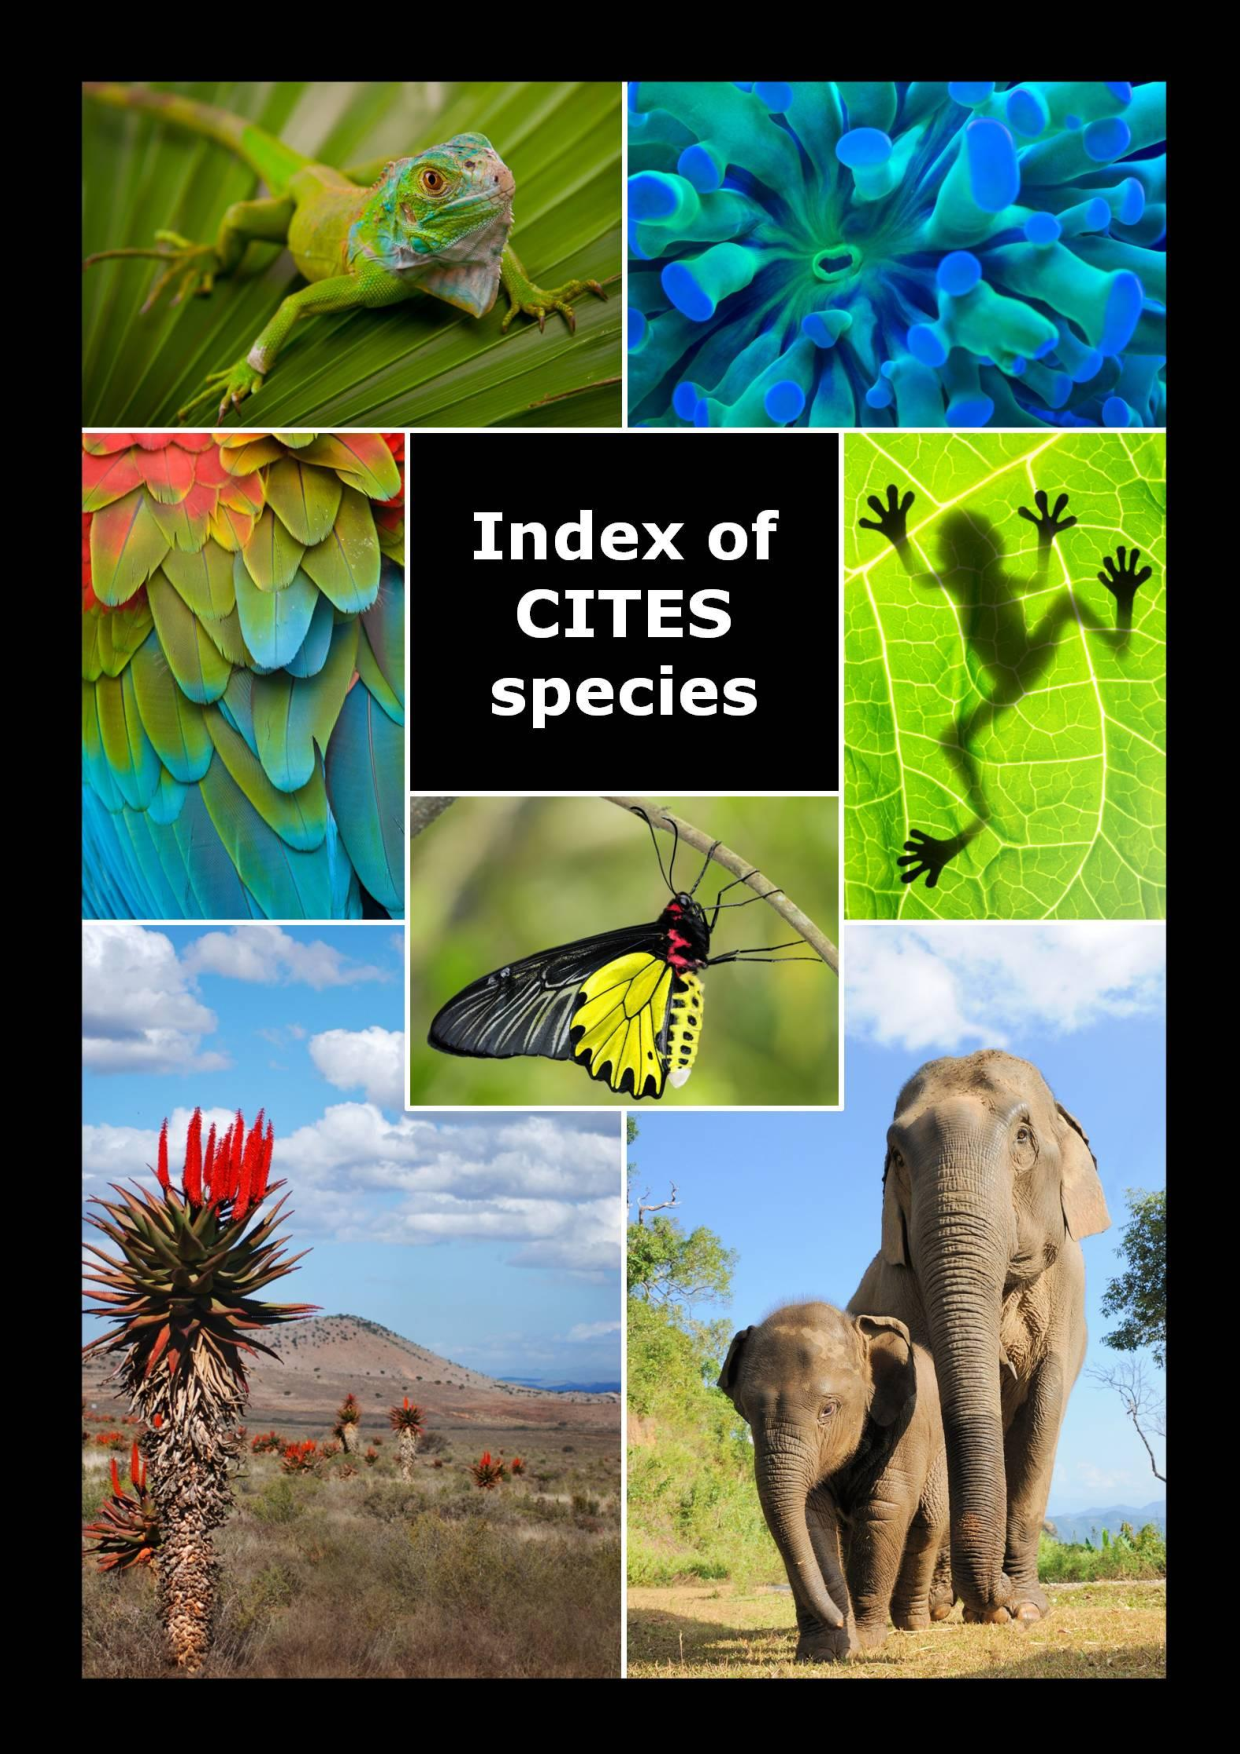
\includepdf[pages={-}]{../../public/latex/static_index.pdf}
\rmfamily
\leftskip 0.1in
\parindent -0.1in

\rmfamily
\csection{INDEX OF FAUNA}

\begin{multicols}{2}{
Put the text here.

Maths, tabulars, pictures etc are all ok (but not
figures and tables).

Remember to load in the \texttt{multicol}
package at the top of your document.

\textbf{\textit{Euphorbia milii} var. \textit{tulearensis}:} \#4 \textbf{II} EUPHORBIACEAE

\textit{Turbinaria irregularis}: \textbf{II} \superscript{39} DENDROPHYLLIIDAE (Anthozoa)

\textit{Turbinaria maxima} = \textit{Turbinaria peltata}

\textit{Turbinaria mesenterina}: II \superscript{39} DENDROPHYLLIIDAE (Anthozoa) (E) Pagoda Coral, Vase Coral

}
\end{multicols}

\subsection{Subsection Heading Here}

Excluding species which are not succulent, and artificially
propagated specimens of cultivars of Euphorbia trigona.
Artificially propagated specimens of Euphorbia spp. are not
subject to the provisions of the Convention when they are of
crested, fan-shaped or colour mutants of E. lactea grafted on
artificially propagated root stock of E. neriifolia, and artificially
propagated specimens of cultivars of E. ‘Milii’ when they are
traded in shipments of 100 or more plants and readily
recognizable as artificially propagated specimens.
Excluidas las especies que no son suculentas, y los
especímenes reproducidos artificialmente de cultivares de
Euphorbia trigona. Los especímenes reproducido
artificialmente, que tengan las ramas crestadas o en forma de
abanico o sean mutantes cromáticos de E. lactea, cuando
estén injertados en rizomas de E. neriifolia reproducidos
artificialmente, y los especímenes reproducidos artificialmente
de cultivares de E. “Milii” cuando se comercialicen en envíos
de 100 o más plantas y se reconozcan fácilmente como
especímenes reproducidos artificialmente, no están sujetos a
las disposiciones de la Convención.
Sauf les espèces non succulentes et les spécimens reproduits
artificiellement de cultivars d'Euphorbia trigona. Les
spécimens reproduits artificiellement de mutants colorés, à
crête ou en éventail d’Euphorbia lactea greffés sur des porte-
greffes reproduits artificiellement d'Euphorbia neriifolia, ainsi
que les spécimens reproduits artificiellement de cultivars
d’Euphorbia “Milii” lorsqu’ils sont commercialisés en envois de
100 plants ou plus et facilement reconnaissables comme étant
des spécimens reproduits artificiellement ne sont pas soumis
aux dispositions de la Convention.
\footnote{Excluding species which are not succulent, and artificially
propagated specimens of cultivars of Euphorbia trigona.
Artificially propagated specimens of Euphorbia spp. are not
subject to the provisions of the Convention when they are of
crested, fan-shaped or colour mutants of E. lactea grafted on
artificially propagated root stock of E. neriifolia, and artificially
propagated specimens of cultivars of E. ‘Milii’ when they are
traded in shipments of 100 or more plants and readily
recognizable as artificially propagated specimens.
Excluidas las especies que no son suculentas, y los
especímenes reproducidos artificialmente de cultivares de
Euphorbia trigona. Los especímenes reproducido
artificialmente, que tengan las ramas crestadas o en forma de
abanico o sean mutantes cromáticos de E. lactea, cuando
estén injertados en rizomas de E. neriifolia reproducidos
artificialmente, y los especímenes reproducidos artificialmente
de cultivares de E. “Milii” cuando se comercialicen en envíos
de 100 o más plantas y se reconozcan fácilmente como
especímenes reproducidos artificialmente, no están sujetos a
las disposiciones de la Convención.
Sauf les espèces non succulentes et les spécimens reproduits
artificiellement de cultivars d'Euphorbia trigona. Les
spécimens reproduits artificiellement de mutants colorés, à
crête ou en éventail d’Euphorbia lactea greffés sur des porte-
greffes reproduits artificiellement d'Euphorbia neriifolia, ainsi
que les spécimens reproduits artificiellement de cultivars
d’Euphorbia “Milii” lorsqu’ils sont commercialisés en envois de
100 plants ou plus et facilement reconnaissables comme étant
des spécimens reproduits artificiellement ne sont pas soumis
aux dispositions de la Convention.
}


\section{Conclusion}

Lorem ipsum dolor sit amet, consectetur adipisicing elit, sed do eiusmod tempor
incididunt ut labore et dolore magna aliqua. Ut enim ad minim veniam, quis
nostrud exercitation ullamco laboris nisi ut aliquip ex ea commodo consequat.
Duis aute irure dolor in reprehenderit in voluptate velit esse cillum dolore eu
fugiat nulla pariatur.


\attachfile[icon=Paperclip]{../../public/latex/CITES_abbreviations_and_annotations.pdf}

\end{document}
